% /home/bougui/source/misc/latex/tikz/3D-rotate-arrow.tex
\documentclass{standalone}
\usepackage{tikz}
\usetikzlibrary{arrows.meta, decorations.markings, calc, fadings,
decorations.pathreplacing, patterns, decorations.pathmorphing, positioning}

\newcommand{\AxisRotator}[1][rotate=0] {%
  \tikz[decoration={
    markings,
    mark=at position 1 with {\arrow{latex}}}]\draw[x = .5em, y = 2.75em, line width = .2ex,#1,postaction=decorate] (0,0)  arc (-150:150:.45 and .5) -- ++(-95:2pt);%                                                   
  }

\begin{document}

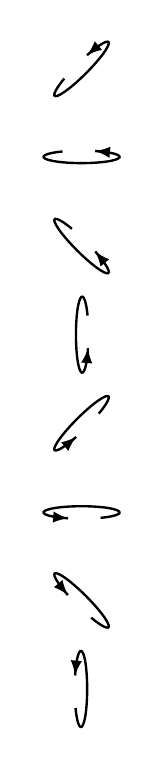
\begin{tikzpicture}[scale = .75]
\foreach \angle[count=\xi] in {0,45,...,315}
  \draw (0,1.5) node at (0,1.5*\xi) {\AxisRotator[rotate = \angle]};
\end{tikzpicture}

\end{document}
